% Options for packages loaded elsewhere
\PassOptionsToPackage{unicode}{hyperref}
\PassOptionsToPackage{hyphens}{url}
\PassOptionsToPackage{dvipsnames,svgnames,x11names}{xcolor}
%
\documentclass[
  letterpaper,
  DIV=11,
  numbers=noendperiod]{scrartcl}

\usepackage{amsmath,amssymb}
\usepackage{lmodern}
\usepackage{iftex}
\ifPDFTeX
  \usepackage[T1]{fontenc}
  \usepackage[utf8]{inputenc}
  \usepackage{textcomp} % provide euro and other symbols
\else % if luatex or xetex
  \usepackage{unicode-math}
  \defaultfontfeatures{Scale=MatchLowercase}
  \defaultfontfeatures[\rmfamily]{Ligatures=TeX,Scale=1}
\fi
% Use upquote if available, for straight quotes in verbatim environments
\IfFileExists{upquote.sty}{\usepackage{upquote}}{}
\IfFileExists{microtype.sty}{% use microtype if available
  \usepackage[]{microtype}
  \UseMicrotypeSet[protrusion]{basicmath} % disable protrusion for tt fonts
}{}
\makeatletter
\@ifundefined{KOMAClassName}{% if non-KOMA class
  \IfFileExists{parskip.sty}{%
    \usepackage{parskip}
  }{% else
    \setlength{\parindent}{0pt}
    \setlength{\parskip}{6pt plus 2pt minus 1pt}}
}{% if KOMA class
  \KOMAoptions{parskip=half}}
\makeatother
\usepackage{xcolor}
\setlength{\emergencystretch}{3em} % prevent overfull lines
\setcounter{secnumdepth}{-\maxdimen} % remove section numbering
% Make \paragraph and \subparagraph free-standing
\ifx\paragraph\undefined\else
  \let\oldparagraph\paragraph
  \renewcommand{\paragraph}[1]{\oldparagraph{#1}\mbox{}}
\fi
\ifx\subparagraph\undefined\else
  \let\oldsubparagraph\subparagraph
  \renewcommand{\subparagraph}[1]{\oldsubparagraph{#1}\mbox{}}
\fi

\usepackage{color}
\usepackage{fancyvrb}
\newcommand{\VerbBar}{|}
\newcommand{\VERB}{\Verb[commandchars=\\\{\}]}
\DefineVerbatimEnvironment{Highlighting}{Verbatim}{commandchars=\\\{\}}
% Add ',fontsize=\small' for more characters per line
\usepackage{framed}
\definecolor{shadecolor}{RGB}{241,243,245}
\newenvironment{Shaded}{\begin{snugshade}}{\end{snugshade}}
\newcommand{\AlertTok}[1]{\textcolor[rgb]{0.68,0.00,0.00}{#1}}
\newcommand{\AnnotationTok}[1]{\textcolor[rgb]{0.37,0.37,0.37}{#1}}
\newcommand{\AttributeTok}[1]{\textcolor[rgb]{0.40,0.45,0.13}{#1}}
\newcommand{\BaseNTok}[1]{\textcolor[rgb]{0.68,0.00,0.00}{#1}}
\newcommand{\BuiltInTok}[1]{\textcolor[rgb]{0.00,0.23,0.31}{#1}}
\newcommand{\CharTok}[1]{\textcolor[rgb]{0.13,0.47,0.30}{#1}}
\newcommand{\CommentTok}[1]{\textcolor[rgb]{0.37,0.37,0.37}{#1}}
\newcommand{\CommentVarTok}[1]{\textcolor[rgb]{0.37,0.37,0.37}{\textit{#1}}}
\newcommand{\ConstantTok}[1]{\textcolor[rgb]{0.56,0.35,0.01}{#1}}
\newcommand{\ControlFlowTok}[1]{\textcolor[rgb]{0.00,0.23,0.31}{#1}}
\newcommand{\DataTypeTok}[1]{\textcolor[rgb]{0.68,0.00,0.00}{#1}}
\newcommand{\DecValTok}[1]{\textcolor[rgb]{0.68,0.00,0.00}{#1}}
\newcommand{\DocumentationTok}[1]{\textcolor[rgb]{0.37,0.37,0.37}{\textit{#1}}}
\newcommand{\ErrorTok}[1]{\textcolor[rgb]{0.68,0.00,0.00}{#1}}
\newcommand{\ExtensionTok}[1]{\textcolor[rgb]{0.00,0.23,0.31}{#1}}
\newcommand{\FloatTok}[1]{\textcolor[rgb]{0.68,0.00,0.00}{#1}}
\newcommand{\FunctionTok}[1]{\textcolor[rgb]{0.28,0.35,0.67}{#1}}
\newcommand{\ImportTok}[1]{\textcolor[rgb]{0.00,0.46,0.62}{#1}}
\newcommand{\InformationTok}[1]{\textcolor[rgb]{0.37,0.37,0.37}{#1}}
\newcommand{\KeywordTok}[1]{\textcolor[rgb]{0.00,0.23,0.31}{#1}}
\newcommand{\NormalTok}[1]{\textcolor[rgb]{0.00,0.23,0.31}{#1}}
\newcommand{\OperatorTok}[1]{\textcolor[rgb]{0.37,0.37,0.37}{#1}}
\newcommand{\OtherTok}[1]{\textcolor[rgb]{0.00,0.23,0.31}{#1}}
\newcommand{\PreprocessorTok}[1]{\textcolor[rgb]{0.68,0.00,0.00}{#1}}
\newcommand{\RegionMarkerTok}[1]{\textcolor[rgb]{0.00,0.23,0.31}{#1}}
\newcommand{\SpecialCharTok}[1]{\textcolor[rgb]{0.37,0.37,0.37}{#1}}
\newcommand{\SpecialStringTok}[1]{\textcolor[rgb]{0.13,0.47,0.30}{#1}}
\newcommand{\StringTok}[1]{\textcolor[rgb]{0.13,0.47,0.30}{#1}}
\newcommand{\VariableTok}[1]{\textcolor[rgb]{0.07,0.07,0.07}{#1}}
\newcommand{\VerbatimStringTok}[1]{\textcolor[rgb]{0.13,0.47,0.30}{#1}}
\newcommand{\WarningTok}[1]{\textcolor[rgb]{0.37,0.37,0.37}{\textit{#1}}}

\providecommand{\tightlist}{%
  \setlength{\itemsep}{0pt}\setlength{\parskip}{0pt}}\usepackage{longtable,booktabs,array}
\usepackage{calc} % for calculating minipage widths
% Correct order of tables after \paragraph or \subparagraph
\usepackage{etoolbox}
\makeatletter
\patchcmd\longtable{\par}{\if@noskipsec\mbox{}\fi\par}{}{}
\makeatother
% Allow footnotes in longtable head/foot
\IfFileExists{footnotehyper.sty}{\usepackage{footnotehyper}}{\usepackage{footnote}}
\makesavenoteenv{longtable}
\usepackage{graphicx}
\makeatletter
\def\maxwidth{\ifdim\Gin@nat@width>\linewidth\linewidth\else\Gin@nat@width\fi}
\def\maxheight{\ifdim\Gin@nat@height>\textheight\textheight\else\Gin@nat@height\fi}
\makeatother
% Scale images if necessary, so that they will not overflow the page
% margins by default, and it is still possible to overwrite the defaults
% using explicit options in \includegraphics[width, height, ...]{}
\setkeys{Gin}{width=\maxwidth,height=\maxheight,keepaspectratio}
% Set default figure placement to htbp
\makeatletter
\def\fps@figure{htbp}
\makeatother

\KOMAoption{captions}{tableheading}
\makeatletter
\@ifpackageloaded{tcolorbox}{}{\usepackage[many]{tcolorbox}}
\@ifpackageloaded{fontawesome5}{}{\usepackage{fontawesome5}}
\definecolor{quarto-callout-color}{HTML}{909090}
\definecolor{quarto-callout-note-color}{HTML}{0758E5}
\definecolor{quarto-callout-important-color}{HTML}{CC1914}
\definecolor{quarto-callout-warning-color}{HTML}{EB9113}
\definecolor{quarto-callout-tip-color}{HTML}{00A047}
\definecolor{quarto-callout-caution-color}{HTML}{FC5300}
\definecolor{quarto-callout-color-frame}{HTML}{acacac}
\definecolor{quarto-callout-note-color-frame}{HTML}{4582ec}
\definecolor{quarto-callout-important-color-frame}{HTML}{d9534f}
\definecolor{quarto-callout-warning-color-frame}{HTML}{f0ad4e}
\definecolor{quarto-callout-tip-color-frame}{HTML}{02b875}
\definecolor{quarto-callout-caution-color-frame}{HTML}{fd7e14}
\makeatother
\makeatletter
\makeatother
\makeatletter
\makeatother
\makeatletter
\@ifpackageloaded{caption}{}{\usepackage{caption}}
\AtBeginDocument{%
\ifdefined\contentsname
  \renewcommand*\contentsname{Table of contents}
\else
  \newcommand\contentsname{Table of contents}
\fi
\ifdefined\listfigurename
  \renewcommand*\listfigurename{List of Figures}
\else
  \newcommand\listfigurename{List of Figures}
\fi
\ifdefined\listtablename
  \renewcommand*\listtablename{List of Tables}
\else
  \newcommand\listtablename{List of Tables}
\fi
\ifdefined\figurename
  \renewcommand*\figurename{Figure}
\else
  \newcommand\figurename{Figure}
\fi
\ifdefined\tablename
  \renewcommand*\tablename{Table}
\else
  \newcommand\tablename{Table}
\fi
}
\@ifpackageloaded{float}{}{\usepackage{float}}
\floatstyle{ruled}
\@ifundefined{c@chapter}{\newfloat{codelisting}{h}{lop}}{\newfloat{codelisting}{h}{lop}[chapter]}
\floatname{codelisting}{Listing}
\newcommand*\listoflistings{\listof{codelisting}{List of Listings}}
\makeatother
\makeatletter
\@ifpackageloaded{caption}{}{\usepackage{caption}}
\@ifpackageloaded{subcaption}{}{\usepackage{subcaption}}
\makeatother
\makeatletter
\@ifpackageloaded{tcolorbox}{}{\usepackage[many]{tcolorbox}}
\makeatother
\makeatletter
\@ifundefined{shadecolor}{\definecolor{shadecolor}{rgb}{.97, .97, .97}}
\makeatother
\makeatletter
\makeatother
\ifLuaTeX
  \usepackage{selnolig}  % disable illegal ligatures
\fi
\IfFileExists{bookmark.sty}{\usepackage{bookmark}}{\usepackage{hyperref}}
\IfFileExists{xurl.sty}{\usepackage{xurl}}{} % add URL line breaks if available
\urlstyle{same} % disable monospaced font for URLs
\hypersetup{
  pdftitle={Інструкція з використання Quarto для підготовки результатів наукових досліджень},
  pdfauthor={Юрій Клебан},
  colorlinks=true,
  linkcolor={blue},
  filecolor={Maroon},
  citecolor={Blue},
  urlcolor={Blue},
  pdfcreator={LaTeX via pandoc}}

\title{Інструкція з використання Quarto для підготовки результатів
наукових досліджень}
\author{Юрій Клебан}
\date{}

\begin{document}
\maketitle
\ifdefined\Shaded\renewenvironment{Shaded}{\begin{tcolorbox}[frame hidden, borderline west={3pt}{0pt}{shadecolor}, boxrule=0pt, sharp corners, enhanced, interior hidden, breakable]}{\end{tcolorbox}}\fi

\begin{tcolorbox}[enhanced jigsaw, coltitle=black, colback=white, opacitybacktitle=0.6, bottomtitle=1mm, colbacktitle=quarto-callout-important-color!10!white, bottomrule=.15mm, opacityback=0, toprule=.15mm, toptitle=1mm, breakable, titlerule=0mm, title=\textcolor{quarto-callout-important-color}{\faExclamation}\hspace{0.5em}{Important}, arc=.35mm, leftrule=.75mm, left=2mm, colframe=quarto-callout-important-color-frame, rightrule=.15mm]
Увага! У тексті публікації зустрічастимуться подібні вставки, вони не є
частиною контенту, а використані для звернення уваги студентів на деякі
моменти підготовки роботи. Не потрібно подібні вставки використовувати
під час написання звіту.
\end{tcolorbox}

\begin{tcolorbox}[enhanced jigsaw, coltitle=black, colback=white, opacitybacktitle=0.6, bottomtitle=1mm, colbacktitle=quarto-callout-color!10!white, bottomrule=.15mm, opacityback=0, toprule=.15mm, toptitle=1mm, breakable, titlerule=0mm, title={Noty}, arc=.35mm, leftrule=.75mm, left=2mm, colframe=quarto-callout-color-frame, rightrule=.15mm]
Зверху справа можна переглянути ``початковий'' код розмітки цього
документа і користуватися ним для підготовки алсної публікації.
\end{tcolorbox}

\begin{center}\rule{0.5\linewidth}{0.5pt}\end{center}

\hypertarget{ux430ux43dux43eux442ux430ux446ux456ux44f}{%
\paragraph{Анотація}\label{ux430ux43dux43eux442ux430ux446ux456ux44f}}

У статті описано процес підготовки матеріалів фінального проєкту з
використанням технології \href{https://quarto.org}{\texttt{Quarto}}.
\texttt{Quarto} дозволяє аналітикам та науковцям обєднати текстові,
графічні матеріали та виконуваний код в один документ.

Увага! Quarto побудовано на основі \texttt{rMarkdown} і відмінності
мінімальні.

\hypertarget{ux43aux43bux44eux447ux43eux432ux456-ux441ux43bux43eux432ux430}{%
\paragraph{Ключові
слова}\label{ux43aux43bux44eux447ux43eux432ux456-ux441ux43bux43eux432ux430}}

\texttt{quarto}, \texttt{r}, \texttt{RStudio\ Desktop},
\texttt{підготовка\ звітів}, \texttt{фінальний\ проєкт}.

\hypertarget{ux43eux441ux43dux43eux432ux43dux430-ux447ux430ux441ux442ux438ux43dux430}{%
\subsection{Основна
частина}\label{ux43eux441ux43dux43eux432ux43dux430-ux447ux430ux441ux442ux438ux43dux430}}

\hypertarget{ux456ux43dux441ux442ux430ux43bux44fux446ux456ux44f}{%
\subsubsection{Інсталяція}\label{ux456ux43dux441ux442ux430ux43bux44fux446ux456ux44f}}

Першим етапом роботи з технологією \texttt{Quarto} є інсталяція. Окрім
уже встановлених на ПК \texttt{R} та \texttt{RStudio} потрібно
завантажиити та виконати кроки зі встановлення
\href{https://quarto.org/docs/get-started/}{\texttt{Quarto\ CLI}}
(\texttt{Command\ Line\ Interface}) для запуску операцій рендерінгу
розмітки та ноутбуків.

Наступний етап передбачає вибір інструменту для написання коду:
\texttt{Visual\ Studio\ Code}, \texttt{RStudio\ Desktop},
\texttt{Jupyter\ Notebook\textbackslash{}Lab} або будь-який текстовий
редактор.

\hypertarget{ux43fux43eux447ux430ux442ux43eux43a-ux440ux43eux431ux43eux442ux438-ux437-ux434ux43eux43aux443ux43cux435ux43dux442ux43eux43c}{%
\subsubsection{Початок роботи з
документом}\label{ux43fux43eux447ux430ux442ux43eux43a-ux440ux43eux431ux43eux442ux438-ux437-ux434ux43eux43aux443ux43cux435ux43dux442ux43eux43c}}

Для початку роботи варто ініціалізувати заголовок документа, вказавши
інформацію про публікацію та автора/ів. Також у заголовку можуть бути
додані додаткові параметри налаштування документа.

\begin{verbatim}
---
title: "Інструкція з використання Quarto для підготовки результатів наукових досліджень"
author: "Юрій Клебан"
format: 
  html:
    code-fold: true # дозволяє отримати згорнутий код
    code-tools: true # додає зверху справа публікації кнопку для перегляду початкового коду розмітки
    code-line-numbers: true # показує номери рядків коду у блоках
execute:
  echo: false # приховує весь код, лишає тільки результати обчислень
---
\end{verbatim}

Зверніть увагу, якщо Ви бажаєте візуалізувати деякі дані, що не мають
виконуваного коду, то варто скористатися записом без \texttt{\{r\}}
(\texttt{на\ початку\ та} вкінці коду):

\begin{verbatim}
# Приклад візуалізації коду "як є".
\end{verbatim}

Якщо ж код має виконуватися, то є кілька варіантів його представлення.

Подібний синтаксис дозволить вивести код і результат у документ.

\begin{Shaded}
\begin{Highlighting}[numbers=left,,]
\NormalTok{x }\OtherTok{\textless{}{-}} \DecValTok{10}
\NormalTok{x}
\end{Highlighting}
\end{Shaded}

\begin{verbatim}
[1] 10
\end{verbatim}

Виведення тільки результату, без коду:

\begin{verbatim}
[1] 10
\end{verbatim}

\begin{tcolorbox}[enhanced jigsaw, coltitle=black, colback=white, opacitybacktitle=0.6, bottomtitle=1mm, colbacktitle=quarto-callout-note-color!10!white, bottomrule=.15mm, opacityback=0, toprule=.15mm, toptitle=1mm, breakable, titlerule=0mm, title=\textcolor{quarto-callout-note-color}{\faInfo}\hspace{0.5em}{Note}, arc=.35mm, leftrule=.75mm, left=2mm, colframe=quarto-callout-note-color-frame, rightrule=.15mm]
Використовуйте \texttt{echo}, адже ми формуємо наукову публікацію, а не
ноутбук!
\end{tcolorbox}

Якщо Вам потрібно прямо у тексті роботи вивести результати обчислень, то
можна скористатися записом типу 3.16 та отримати 3.16, тобто очислення
будуь відбуватися ``на льоту''.

\hypertarget{ux43eux444ux43eux440ux43cux43bux435ux43dux43dux44f-ux442ux435ux43aux441ux442ux456ux432}{%
\subsubsection{Оформлення
текстів}\label{ux43eux444ux43eux440ux43cux43bux435ux43dux43dux44f-ux442ux435ux43aux441ux442ux456ux432}}

Оформлення текствої інформації

\hypertarget{ux43fux443ux431ux43bux456ux43aux430ux446ux456ux44f-ux437ux43eux431ux440ux430ux436ux435ux43dux44c}{%
\subsubsection{Публікація
зображень}\label{ux43fux443ux431ux43bux456ux43aux430ux446ux456ux44f-ux437ux43eux431ux440ux430ux436ux435ux43dux44c}}

\hypertarget{ux442ux430ux431ux43bux438ux447ux43dux435-ux43fux440ux435ux434ux441ux442ux430ux432ux43bux435ux43dux43dux44f-ux434ux430ux43dux438ux445}{%
\subsubsection{Табличне представлення
даних}\label{ux442ux430ux431ux43bux438ux447ux43dux435-ux43fux440ux435ux434ux441ux442ux430ux432ux43bux435ux43dux43dux44f-ux434ux430ux43dux438ux445}}

Візуалізація табличної інформації може бути представлена двома
способами:

-{[}x{]} у вигляді розмітки;

-{[}x{]} візуалізація датафрейму.

\begin{verbatim}
| fruit  | price  |
|--------|--------:
| apple  | 2.05   |
| pear   | 1.37   |
| orange | 3.09   |

: Ціна на фрукти {tbl-colwidths="[60,40]"}
\end{verbatim}

Для публікації інформації з наявного датафрейму можна використовувати
використати звичайну виведення:

\begin{Shaded}
\begin{Highlighting}[numbers=left,,]
\NormalTok{  mtcars[}\DecValTok{1}\SpecialCharTok{:}\DecValTok{3}\NormalTok{, }\DecValTok{1}\SpecialCharTok{:}\DecValTok{5}\NormalTok{]}
\end{Highlighting}
\end{Shaded}

\begin{verbatim}
               mpg cyl disp  hp drat
Mazda RX4     21.0   6  160 110 3.90
Mazda RX4 Wag 21.0   6  160 110 3.90
Datsun 710    22.8   4  108  93 3.85
\end{verbatim}

Проте візуально інформацію зручніше візуалізувати за допомогою функції
\texttt{knitr::kable()} та з використання спеціальних підписів у
заголовку коду:

\begin{Shaded}
\begin{Highlighting}[numbers=left,,]
\NormalTok{knitr}\SpecialCharTok{::}\FunctionTok{kable}\NormalTok{(}
\NormalTok{  mtcars[}\DecValTok{1}\SpecialCharTok{:}\DecValTok{3}\NormalTok{, }\DecValTok{1}\SpecialCharTok{:}\DecValTok{5}\NormalTok{]}
\NormalTok{)}
\end{Highlighting}
\end{Shaded}

\begin{table}

\caption{Назва таблиці}\begin{minipage}[t]{\linewidth}
\subcaption{\label{tbl-anonymous-7994095-1}Джерело: дані з пакету
carData}

{\centering 

\begin{tabular}[t]{lrrrrr}
\toprule
 & mpg & cyl & disp & hp & drat\\
\midrule
Mazda RX4 & 21.0 & 6 & 160 & 110 & 3.90\\
Mazda RX4 Wag & 21.0 & 6 & 160 & 110 & 3.90\\
Datsun 710 & 22.8 & 4 & 108 & 93 & 3.85\\
\bottomrule
\end{tabular}

}

\end{minipage}%

\end{table}

\hypertarget{ux43fux43eux431ux443ux434ux43eux432ux430-ux434ux456ux430ux433ux440ux430ux43c-ux442ux430-ux433ux440ux430ux444ux456ux43aux456ux432}{%
\subsubsection{Побудова діаграм та
графіків}\label{ux43fux43eux431ux443ux434ux43eux432ux430-ux434ux456ux430ux433ux440ux430ux43c-ux442ux430-ux433ux440ux430ux444ux456ux43aux456ux432}}

\begin{figure}

{\centering 

\begin{Shaded}
\begin{Highlighting}[numbers=left,,]
\FunctionTok{library}\NormalTok{(ggplot2)}
\NormalTok{mtcars2 }\OtherTok{\textless{}{-}}\NormalTok{ mtcars}
\NormalTok{mtcars2}\SpecialCharTok{$}\NormalTok{am }\OtherTok{\textless{}{-}} \FunctionTok{factor}\NormalTok{(}
\NormalTok{  mtcars}\SpecialCharTok{$}\NormalTok{am, }\AttributeTok{labels =} \FunctionTok{c}\NormalTok{(}\StringTok{\textquotesingle{}automatic\textquotesingle{}}\NormalTok{, }\StringTok{\textquotesingle{}manual\textquotesingle{}}\NormalTok{)}
\NormalTok{)}
\FunctionTok{ggplot}\NormalTok{(mtcars2, }\FunctionTok{aes}\NormalTok{(hp, mpg, }\AttributeTok{color =}\NormalTok{ am)) }\SpecialCharTok{+}
  \FunctionTok{geom\_point}\NormalTok{() }\SpecialCharTok{+}  \FunctionTok{geom\_smooth}\NormalTok{(}\AttributeTok{formula =}\NormalTok{ y }\SpecialCharTok{\textasciitilde{}}\NormalTok{ x, }\AttributeTok{method =} \StringTok{"loess"}\NormalTok{) }\SpecialCharTok{+}
  \FunctionTok{theme}\NormalTok{(}\AttributeTok{legend.position =} \StringTok{\textquotesingle{}bottom\textquotesingle{}}\NormalTok{)}
\end{Highlighting}
\end{Shaded}

\begin{figure}[H]

{\centering 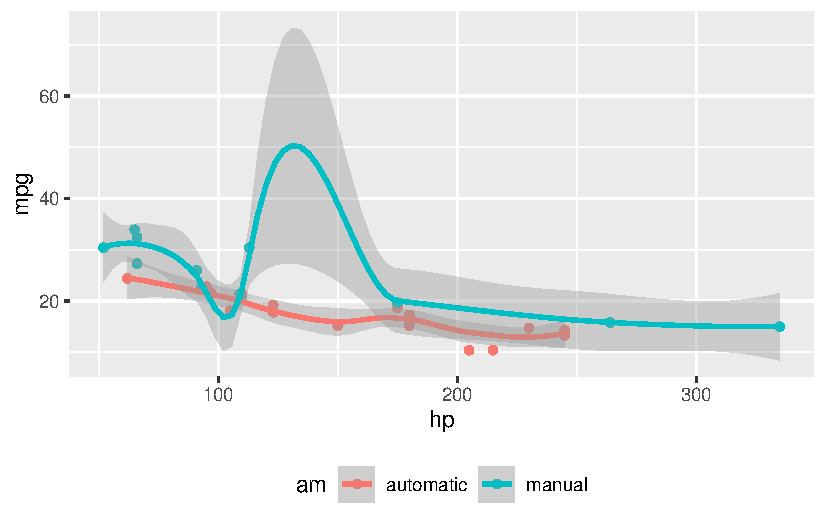
\includegraphics{quarto-tutorial_files/figure-pdf/fig-cap-margin-1.pdf}

}

\caption{Дані з пакету \texttt{CarData}}

\end{figure}

}

\caption{\label{fig-cap-margin}MPG vs horsepower, colored by
transmission.}

\end{figure}

\hypertarget{ux444ux43eux440ux43cux443ux43bux438-ux442ux430-ux447ux438ux441ux43bux43eux432ux456-ux43fux43eux437ux43dux430ux447ux435ux43dux43dux44f}{%
\subsubsection{Формули та числові
позначення}\label{ux444ux43eux440ux43cux443ux43bux438-ux442ux430-ux447ux438ux441ux43bux43eux432ux456-ux43fux43eux437ux43dux430ux447ux435ux43dux43dux44f}}

\hypertarget{ux432ux438ux441ux43dux43eux432ux43aux438}{%
\subsection{Висновки}\label{ux432ux438ux441ux43dux43eux432ux43aux438}}

\hypertarget{ux441ux43fux438ux441ux43eux43a-ux432ux438ux43aux43eux440ux438ux441ux442ux430ux43dux438ux445-ux434ux436ux435ux440ux435ux43b}{%
\subsection{Список використаних
джерел}\label{ux441ux43fux438ux441ux43eux43a-ux432ux438ux43aux43eux440ux438ux441ux442ux430ux43dux438ux445-ux434ux436ux435ux440ux435ux43b}}

\begin{enumerate}
\def\labelenumi{\arabic{enumi}.}
\tightlist
\item
  https://quarto.org/
\end{enumerate}

\begin{Shaded}
\begin{Highlighting}[numbers=left,,]
\DecValTok{1} \SpecialCharTok{+} \DecValTok{1}
\end{Highlighting}
\end{Shaded}

\begin{verbatim}
[1] 2
\end{verbatim}



\end{document}
